\documentclass{article}

% packages
\usepackage{amsmath, amsthm, thmtools, amsfonts, amssymb, luacode, catchfile, tikzducks, hyperref, ifthen}
\ifcsname c@kobocompile\endcsname
	\usepackage[a5paper, total={1072pt, 1448pt}, margin=10pt, includeheadfoot]{geometry} % set page margins
\else
	\usepackage[a4paper, margin=50pt, includeheadfoot]{geometry}
\fi
\usepackage[shortlabels]{enumitem}
\usepackage[skip=3pt, indent=0pt]{parskip}

% language
\usepackage[bidi=basic, layout=tabular, provide=*]{babel}
\ifcsname c@english\endcsname
	\babelprovide[main, import]{english}
\else
	\babelprovide[main, import]{hebrew}
	\babelprovide{rl}
\fi
%\babelfont{rm}{Libertinus Serif}
\babelfont{rm}[Renderer=Harfbuzz]{Libertinus Serif}
\babelfont{sf}{Libertinus Sans}
\babelfont{tt}{Libertinus Mono}

% style
\AddToHook{cmd/section/before}{\clearpage}	% Add line break before section
\linespread{1.3}
\setcounter{secnumdepth}{0}		% Remove default number tags from sections, this won't do well with theorems
\AtBeginDocument{\setlength{\belowdisplayskip}{3pt}}
\AtBeginDocument{\setlength{\abovedisplayskip}{3pt}}
\graphicspath{ {../images/} }

% operators
\DeclareMathOperator\cis{cis}
\DeclareMathOperator\Sp{Sp}
\DeclareMathOperator\tr{tr}
\DeclareMathOperator\im{Im}
\DeclareMathOperator\re{Re}
\DeclareMathOperator\diag{diag}
\DeclareMathOperator*\lowlim{\underline{lim}}
\DeclareMathOperator*\uplim{\overline{lim}}
\DeclareMathOperator\rng{rng}
\DeclareMathOperator\Sym{Sym}
\DeclareMathOperator\Arg{Arg}
\DeclareMathOperator\Log{Log}
\DeclareMathOperator\dom{dom}
\DeclareMathOperator\supp{Supp}
\DeclareMathOperator\var{Var}
\DeclareMathOperator\cov{Cov}

% commands
%\renewcommand\qedsymbol{\textbf{מש''ל}}
%\renewcommand\qedsymbol{\fbox{\emoji{lizard}}}
\newcommand{\Aa}[0]{\mathcal{A}}
\newcommand{\Bb}[0]{\mathcal{B}}
\newcommand{\CC}[0]{\mathbb{C}}
\newcommand{\Cc}[0]{\mathcal{C}}
\newcommand{\EE}[0]{\mathbb{E}}
\newcommand{\FF}[0]{\mathbb{F}}
\newcommand{\Ff}[0]{\mathcal{F}}
\newcommand{\Ii}[0]{\mathcal{I}}
\newcommand{\Gg}[0]{\mathcal{G}}
\newcommand{\Ll}[0]{\mathcal{L}}
\newcommand{\Mm}[0]{\mathcal{M}}
\newcommand{\NN}[0]{\mathbb{N}}
\newcommand{\Nn}[0]{\mathcal{N}}
\newcommand{\PP}[0]{\mathbb{P}}
\newcommand{\Pp}[0]{\mathcal{P}}
\newcommand{\QQ}[0]{\mathbb{Q}}
\newcommand{\RR}[0]{\mathbb{R}}
\newcommand{\Rr}[0]{\mathcal{R}}
\newcommand{\Ss}[0]{\mathcal{S}}
\newcommand{\TT}[0]{\mathbb{T}}
\newcommand{\Uu}[0]{\mathcal{U}}
\newcommand{\Vv}[0]{\mathcal{V}}
\newcommand{\Ww}[0]{\mathcal{W}}
\newcommand{\ZZ}[0]{\mathbb{Z}}
\newcommand{\acts}[0]{\circlearrowright}
\newcommand{\explain}[2] {
	\begin{flalign*}
		 && \text{#2} && \text{#1}
	\end{flalign*}
}
\newcommand{\maketitleprint}[0]{ \begin{center}
	%\begin{tikzpicture}[scale=3]
	%	\duck[graduate=gray!20!black, tassel=red!70!black]
	%\end{tikzpicture}	
	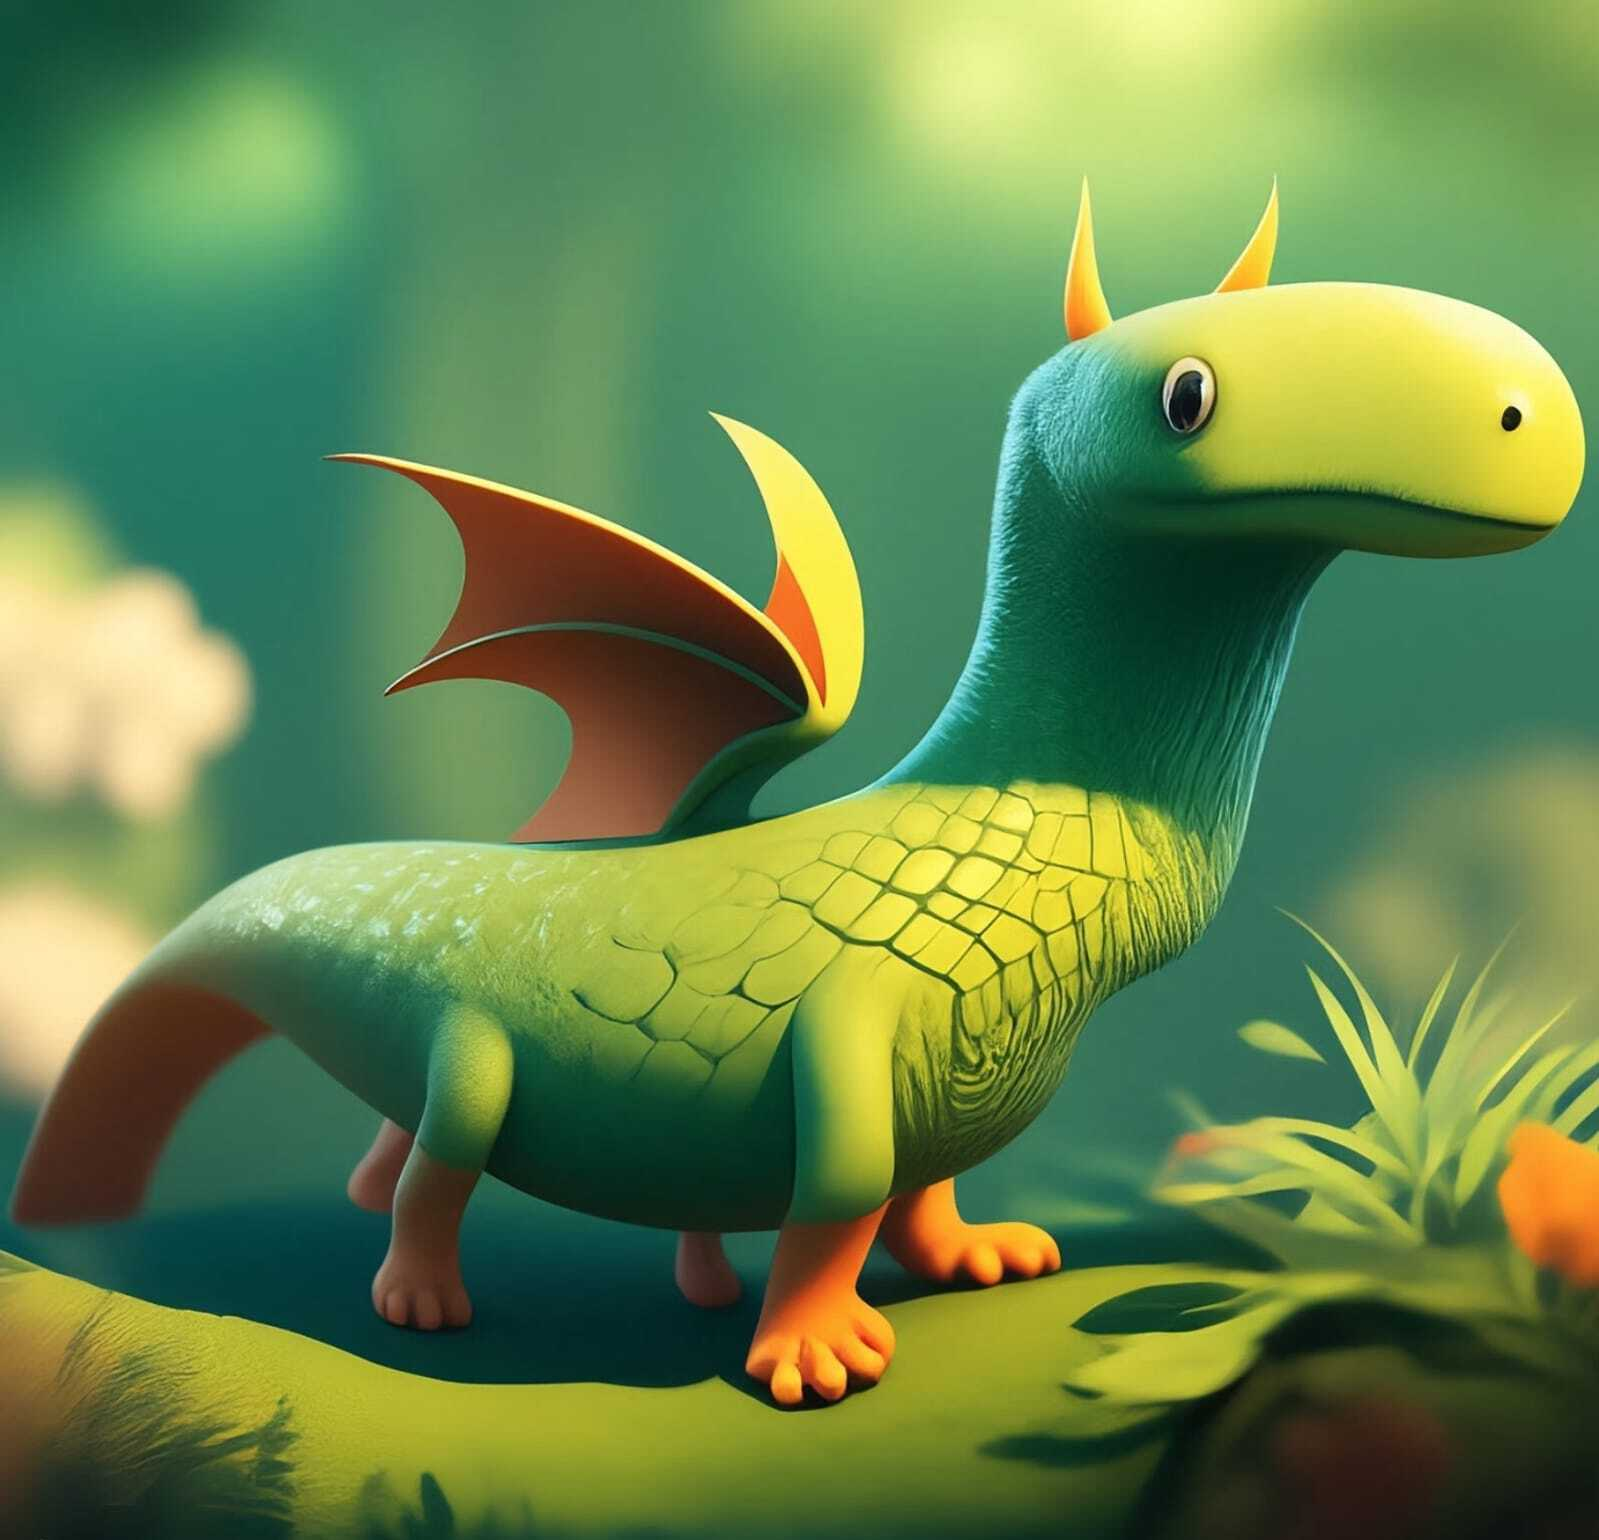
\includegraphics[width=6cm]{cover}
\end{center}
}

% theorem commands
\newtheoremstyle{c_remark}
	{}	% Space above
	{}	% Space below
	{}% Body font
	{}	% Indent amount
	{\bfseries}	% Theorem head font
	{}	% Punctuation after theorem head
	{.5em}	% Space after theorem head
	{\thmname{#1}\thmnumber{ #2}\thmnote{ \normalfont{\text{(#3)}}}}	% head content
\newtheoremstyle{c_definition}
	{3pt}	% Space above
	{3pt}	% Space below
	{}% Body font
	{}	% Indent amount
	{\bfseries}	% Theorem head font
	{}	% Punctuation after theorem head
	{.5em}	% Space after theorem head
	{\thmname{#1}\thmnumber{ #2}\thmnote{ \normalfont{\text{(#3)}}}}	% head content
\newtheoremstyle{c_plain}
	{3pt}	% Space above
	{3pt}	% Space below
	{\itshape}% Body font
	{}	% Indent amount
	{\bfseries}	% Theorem head font
	{}	% Punctuation after theorem head
	{.5em}	% Space after theorem head
	{\thmname{#1}\thmnumber{ #2}\thmnote{ \text{(#3)}}}	% head content

\ifcsname c@english\endcsname
	\theoremstyle{plain}
	\newtheorem{theorem}{Theorem}[section]
	\newtheorem{lemma}[theorem]{Lemma}
	\newtheorem{proposition}[theorem]{Proposition}
	\newtheorem*{proposition*}{Proposition}
	%\newtheorem{corollary}[theorem]{אין חלופה עברית}

	\theoremstyle{definition}
	\newtheorem{definition}[theorem]{Definition}
	\newtheorem*{definition*}{Definition}
	\newtheorem{example}{Example}[section]
	\newtheorem{exercise}{Exercise}[section]

	\theoremstyle{remark}
	\newtheorem*{remark}{Remark}
	\newtheorem*{solution}{Solution}
	\newtheorem{conclusion}[theorem]{Conclusion}
	\newtheorem{notation}[theorem]{Notation}
\else
	\theoremstyle{c_plain}
	\newtheorem{theorem}{משפט}[section]
	\newtheorem{lemma}[theorem]{למה}
	\newtheorem{proposition}[theorem]{טענה}
	\newtheorem*{proposition*}{טענה}
	%\newtheorem{corollary}[theorem]{אין חלופה עברית}

	\theoremstyle{c_definition}
	\newtheorem{definition}[theorem]{הגדרה}
	\newtheorem*{definition*}{הגדרה}
	\newtheorem{example}{דוגמה}[section]
	\newtheorem{exercise}{תרגיל}[section]

	\theoremstyle{c_remark}
	\newtheorem*{remark}{הערה}
	\newtheorem*{solution}{פתרון}
	\newtheorem{conclusion}[theorem]{מסקנה}
	\newtheorem{notation}[theorem]{סימון}
\fi

% Questions related commands
\newcounter{question}
\setcounter{question}{1}
\newcounter{sub_question}
\setcounter{sub_question}{1}

\ifcsname c@english\endcsname
	\newcommand{\question}[1][0]{
		\ifthenelse{#1 = 0}{}{\setcounter{question}{#1}}
		\section{Question \arabic{question}}
		\addtocounter{question}{1}
		\setcounter{sub_question}{1}
	}

	\newcommand{\subquestion}[1][0]{
		\ifthenelse{#1 = 0}{}{\setcounter{sub_question}{#1}}
		\subsection{Part \alph{sub_question}}
		\addtocounter{sub_question}{1}
	}
\else
	\newcommand{\question}[1][0]{
		\ifthenelse{#1 = 0}{}{\setcounter{question}{#1}}
		\section{שאלה \arabic{question}}
		\addtocounter{question}{1}
		\setcounter{sub_question}{1}
	}

	\newcommand{\subquestion}[1][0]{
		\ifthenelse{#1 = 0}{}{\setcounter{sub_question}{#1}}
		\subsection{סעיף \localecounter{letters.gershayim}{sub_question}}
		\addtocounter{sub_question}{1}
	}
\fi

% import lua and start of document
\directlua{common = require ('../common')}

\GetEnv{AUTHOR}

% headers
\author{\AUTHOR}
\date\today

\title{פתרון ממ''ן 13 – אלגברה לינארית 2 (20229)}

\begin{document}
\maketitle

\section{שאלה 1}
יהי $V = M_{n \times n}^\RR$ ותהי $f: V \times V \to \RR$ אשר מוגדרת $f(A, B) = \tr(A^t M B)$ לכל $A, B \in V$.

\subsection{סעיף א'}
נמצא תנאי מספיק והכרחי על $M$ כך ש־$f$ תהיה תבנית סימטרית. \\*
על־פי שאלה 4.1.2 ההעתקה $f$ היא בילינארית. נראה כי
\[
	f(A, B) = \tr(A^t M B) = \tr( {(A^t M B)}^t ) = \tr( {(M B)}^t A) = \tr( B^t M^t A)
\]
אילו הייתה $M$ סימטרית אז $M = M^t$ ובהתאם גם
\[
	\tr(B^t M^t A) = \tr( B^t M A) = f(A, B) = f(B, A)
\]
דהינו, תנאי מספק והכרחי כדי ש־$f$ תהיה תבנית סימטרית הוא ש־$M$ תהיה מטריצה סימטרית.

\subsection{סעיף ב'}
נגדיר $n = 2$, $E$ הבסיס הסטנדרטי של $V$,
\[
	M = \begin{pmatrix}
		1 & 2 \\
		3 & 5
	\end{pmatrix}
\]
נמצא את ${[f]}_E$: \\*
על־פי שאלה 4.1.13 מתקיים
\[
	{[f]}_E = \begin{pmatrix}
		1 & 0 & 2 & 0 \\
		0 & 1 & 0 & 2 \\
		3 & 0 & 5 & 0 \\
		0 & 3 & 0 & 5 \\
	\end{pmatrix}
\]

\subsection{סעיף ג'}
נמצא הצגה של $f$ כסכום של תבנית בילינארית סימטרית ותבנית בילינארית אנטיסימטרית עבור הנתונים אשר הוגדרו בסעיף הקודם. \\*
נגדיר
\begin{align*}
	g_1(A, B) = \frac{1}{2} (f(A, B) + f(B, A)), && g_2(B, A) = \frac{1}{2}(f(A, B) - f(B, A))
\end{align*}
על־פי שאלה 4.2.3 $g_1, g_2$ הן תבניות בילינאריות סימטרית ואנטיסימטרית בהתאמה, ומחישוב ישיר מתקבל כי
\[
	f = g_1 + g_2
\]

\section{שאלה 2}
נוכיח כי תבנית בילינארית $f \ne 0$ ניתנת להצגה כמכפלה של שתי תבניות לינאריות:
\[
	f(x, y) = \left( \sum_{i = 1}^n b_i x_i \right) \left(\sum_{j = 1}^n c_j y_j \right)
\]
אם ורק אם הדרגה של $f$ היא $1$, נסמן גם $\rho f = 1$.
\begin{proof}
	נניח כי $f$ ניתנת להצגה כמכפלת שתי תבניות לינאריות כפי כמתואר לעיל בבסיס נתון ונוכיח כי $\rho f = 1$. \\*
	נגדיר את הבסיס $W = (w_1, w_2, \hdots, w_n)$, אז המטריצה המייצגת את $f$ היא
	\[
		{[f]}_W = \begin{pmatrix}
			b_1 c_1 & b_1 c_2 & \cdots & b_1 c_n \\
			b_2 c_1 & b_2 c_2 & \cdots & b_2 c_n \\
			\vdots & & \ddots & \vdots \\
			b_n c_1 & b_n c_2 & \cdots & b_n c_n \\
		\end{pmatrix}
	\]
	ניתן לראות כי כלל השורות תלויות לינארית, ואנו יודעים כי חייבת להיות לפחות שורה אחת שונה מאפס (שאם לא כן $f = 0$) ולכן $\rho f = 1$. \\*
	נניח כי $\rho f = 1$ ונוכיח כי קיימות שתי תבניות לינאריות עבורן $f$ היא מכפלתן. \\*
	מדרגה זו נובע כי קיים בסיס $W$ עבורו ${[f]}_W$ היא מטריצה בה כלל השורות תלויות לינארית בווקטור יחיד, נסמנו ב־$b$,
	ונגדיר $(c_n)$ סדרת סקלרים אשר מהווים המקדמים של הווקטור במטריצת הייצוג
	\[
		{[f]}_W = \begin{pmatrix}
			b_1 c_1 & \cdots & b_1 c_n \\
			\vdots & \ddots & \vdots \\
			b_n c_1 & \cdots & b_n c_n \\
		\end{pmatrix}
	\]
	ובהתאם לפי מסקנה 4.1.6 מתקיים
	\[
		f(x, y)
		= {[x]}_W {[f]}_W {[y]}_W
		= \sum_{i = 1}^n \sum_{j = 1}^n b_i x_i c_j y_j
		= \left( \sum_{i = 1}^n b_i x_i \right) \left(\sum_{j = 1}^n c_j y_j \right)
	\]
\end{proof}

\section{שאלה 3}
תהי תבנית על $\RR^2$ המוגדרת על־ידי:
\[
	f\left( (x_1, x_2), (y_1, y_2) \right) = x_1 y_1 + 4 x_2 y_2 + 2 x_1 y_2 + 2x_2 y_1
\]

\subsection{סעיף א'}
נוכיח כי $f$ תבנית בילינארית. \\*
מטענה 4.1.4 נובע ש־$f$ תבנית בילינארית, ונבנה לה מטריצת ייצוג:
\[
	A = \begin{pmatrix}
		1 & 2 \\
		2 & 4
	\end{pmatrix}
\]
מלמה 4.2.2 נובע ש־$f$ תבנית סימטרית.
נמצא בסיס בו $f$ מיוצגת על־ידי מטריצה אלכסונית. \\*
התבנית הריבועית המסומכת ל־$f$ היא
\[
	q(x) = f(x, x) = f((x_1, x_2), (x_1, x_2)) = x_1^2 + 4x_1 x_2 + 4 x_2^2 = {(x_1 + 2x_2)}^2
\]
נגדיר משתנה חדש $z \in \RR^2$, על־פי ערך $q$ נגדיר $z_1 = x_1 + 2x_2$, ולכן בהתאם $q(z) = z_1^2 + 0z_2$.
נבחר $z_2 = x_2$ ונראה כי
\[
	f(z, z') = z_1 z'_1
\]
בהתאם מטריצת הייצוג לפי $z$ של $f$ היא
\[
	B = \begin{pmatrix}
		1 & 0 \\
		0 & 0
	\end{pmatrix}
\]
נגדיר $W$ הבסיס שמקיים ${[f]}_W = B$. אז מטריצת המעבר מהבסיס הסטנדרטי ל־$W$ היא לפי שיטת לגרנז':
\[
	M = \begin{pmatrix}
		1 & 2 \\
		0 & 1
	\end{pmatrix}
\]
מחישוב עולה כי $x_2 = z_2$ וכי $x_1 = z_1 - 2z_2$ ולכן בהתאם
\[
	M^{-1} = \begin{pmatrix}
		1 & -2 \\
		0 & 1
	\end{pmatrix}
\]
ובהתאם להגדרת מטריצת המעבר גם $W = ((1, 0), (-2, 1))$.

\subsection{סעיף ב'}
נבדוק את נכונות נוסחת המעבר מן הבסיס הסטנדרטי של $\RR^2$ ל־$W$. \\*
על־פי משפט 4.5.1 התבנית $f$ מקיימת
\[
	A = {[f]}_E = M^t {[f]}_W M = M^t B M
\]
נציב:
\[
	\begin{pmatrix}
		1 & 2 \\
		2 & 4
	\end{pmatrix}
	=
	\begin{pmatrix}
		1 & 0 \\
		2 & 1
	\end{pmatrix}
	\begin{pmatrix}
		1 & 0 \\
		0 & 0
	\end{pmatrix}
	\begin{pmatrix}
		1 & 2 \\
		0 & 1
	\end{pmatrix}
\]
שוויון זה אכן מתקיים בחישוב ישיר, ולכן בהתאם נוסחת המעבר על־ידי שימוש במטריצת המעבר $M$ נכונה.

\section{שאלה 4}
\subsection{סעיף א'}
תהי תבנית ריבועית $q: \RR^n \to \RR$ כאשר $n \in \NN$ המוגדרת על־ידי
\[
	q(x_1, x_2, \ldots, x_n) = \sum_{i = 1}^n x_i^2 + \sum_{1 \le i < j \le n} x_i x_j
\]
נמצא ל־$q$ תבנית אלכסונית. \\*
נגדיר ${[q]}_E = A$ מטריצת ייצוג סימטרית לפי הבסיס הסטנדרטי של $\RR^n$, מהגדרת $q$ נובע:
\[
	A = \begin{pmatrix}
		1  & \frac{1}{2} & \frac{1}{2} & \hdots \\
		\frac{1}{2} & 1 & \frac{1}{2} & \hdots \\
		\frac{1}{2} & \frac{1}{2} & 1 & \hdots \\
		\vdots & & \ddots & \ddots
	\end{pmatrix}
\]
בשל היות המטריצה $A$ סימטרית אז אנו יודעים כי היא חופפת למטריצה אלכסונית, וחפיפה בממשיים מתלכדת עם דמיון אורתוגונלי, נחשב את ערכיה העצמיים של $A$:
\begin{align*}
	& \begin{vmatrix}
		t - 1  & -\frac{1}{2} & -\frac{1}{2} & \hdots \\
		-\frac{1}{2} & t - 1 & -\frac{1}{2} & \hdots \\
		-\frac{1}{2} & -\frac{1}{2} & t - 1 & \hdots \\
		\vdots & & \ddots & \ddots
	\end{vmatrix}
	\xrightarrow{R_1 \to R_1 + \sum_{i = 2}^n R_i}
	\begin{vmatrix}
		t - \frac{n + 1}{2} & t - \frac{n + 1}{2} & t - \frac{n + 1}{2} & \hdots \\
		-\frac{1}{2} & t - 1 & -\frac{1}{2} & \hdots \\
		-\frac{1}{2} & -\frac{1}{2} & t - 1 & \hdots \\
		\vdots & & \ddots & \ddots
	\end{vmatrix} \\
	& \rightarrow
	\left(t - \frac{n + 1}{2}\right)
	\begin{vmatrix}
		1 & 1 & 1 & \cdots \\
		-\frac{1}{2} & t - 1 & -\frac{1}{2} & \hdots \\
		-\frac{1}{2} & -\frac{1}{2} & t - 1 & \hdots \\
		\vdots & & \ddots & \ddots
	\end{vmatrix}
	\xrightarrow{R_i \to R_i + R_1/2 \mid 1 < i \le n}
	\left(t - \frac{n + 1}{2}\right)
	\begin{vmatrix}
		1 & 1 & 1 & \cdots \\
		0 & t - \frac{1}{2} & 0 & \hdots \\
		0 & 0 & t - \frac{1}{2} & \hdots \\
		\vdots & & \ddots & \ddots
	\end{vmatrix} \\
	& \rightarrow
	\left(t - \frac{n + 1}{2}\right)
{\left(t - \frac{1}{2}\right)}^{n - 1}
\end{align*}
אז כלל ערכיה העצמיים הם $\frac{n + 1}{2}, \frac{1}{2}$.
נוכל בדרך דומה לתהליך מציאת הערך העצמי $\frac{n + 1}{2}$ להגיע למסקנה כי $(1, 1, \hdots)$ וקטור עצמי של הערך. \\*
נחשב את המרחב העצמי של $\frac{1}{2}$:
\[
	A x = \frac{1}{2} x
\]
ובהמרה למערכת משוואות הומוגנית
\[
	\begin{pmatrix}
		\frac{1}{2} & \frac{1}{2} & \frac{1}{2} & \hdots \\
		\frac{1}{2} & \frac{1}{2} & \frac{1}{2} & \hdots \\
		\frac{1}{2} & \frac{1}{2} & \frac{1}{2} & \hdots \\
		\vdots & & \ddots & \ddots
	\end{pmatrix}
	\rightarrow
	\begin{pmatrix}
		\frac{1}{2} & \frac{1}{2} & \frac{1}{2} & \hdots \\
		0 & 0 & 0 & \hdots \\
		0 & 0 & 0 & \hdots \\
		\vdots & & \ddots & \ddots
	\end{pmatrix}
	\rightarrow
	\Sp\{ (1, 0, 0, \hdots, -1), (0, 1, 0, \hdots, -1), \hdots, (0, 0, 0, \hdots, 1, -1) \}
\]
קל לבדוק כי מצאנו $n$ וקטורים בלתי תלויים, ולכן $A$ חופפת למטריצה האלכסונית
\[
	\begin{pmatrix}
		\frac{n + 1}{2}  & 0 & 0 & \hdots \\
		0 & \frac{1}{2} & 0 & \hdots \\
		0 & 0 & \frac{1}{2} & \hdots \\
		\vdots & & \ddots & \ddots
	\end{pmatrix}
\]
נמצא תבנית בילינארית סימטרית הקוטבית ל־$q$. \\*
למעשה, המטריצה $A$ כבר מייצגת העתקה כזו:
\[
	p(x, y) = \frac{n + 1}{2} x_1 y_1 + \frac{1}{2} x_2 y_2 + \cdots + \frac{1}{2} x_n y_n
\]

\subsection{סעיף ב'}
נמצא בסיס שבו התבנית הריבועית $q$ היא בעלת צורה אלכסונית. \\*
בסעיף הקודם מצאנו מטריצה אלכסונית כמו גם ערכים עצמיים ווקטורים עצמיים שלהם, של מטריצת הייצוג של התבנית. \\*
כדי למצוא מטריצת לכסון אוניטרית נצטרך למצוא גם בסיס אורתונורמלי מתאים, אותו נוכל לבנות מהבסיס הקיים:
\[
	B = \left( (1, 1, \hdots), (1, 0, 0, \hdots, -1) \hdots \right)
\]
נגדיר $u_i$ הווקטור הנורמלי ה־$i$.
\[
	u_1 = \frac{b_1}{\lVert b_1 \rVert} = \frac{1}{\sqrt{n}} (1, 1, \hdots)
\]
נשים לב כי הווקטור הראשון אורתוגונלי לכל שאר הווקטורים, לכן כדי לנרמל את הבסיס נוכל לבצע הליך גרם־שמידט רק לווקטורים העצמיים של $\frac{1}{2}$.
\[
	u_2 = \frac{b_2}{\lVert b_2 \rVert} = \frac{1}{\sqrt{2}} \left(1, 0, 0, \hdots, -1\right)
	= \left(\frac{1}{\sqrt{2}}, 0, 0, \hdots, \frac{-1}{\sqrt{2}}\right)
\]
נשים לב כי מכפלת כל שני ווקטורים עצמיים שונים של $\frac{1}{2}$ היא $1$ בשל האיבר המשותף האחרון שלהם וחוסר התלות ללא התיחסות אליו.
\begin{align*}
	& v_3 = (0, 1, 0, \hdots, -1) - \frac{1}{\sqrt{2}} u_2 = (-\frac{1}{2}, 1, 0, \hdots, -\frac{1}{2}) \\
	& u_3 = \frac{v_3}{\lVert v_3 \rVert} = \frac{\sqrt{2}}{\sqrt{3}} u_2 = \frac{1}{\sqrt{6}} (-1, 2, 0, \hdots, -1)
\end{align*}
ניתן להוכיח באינדוקציה שהביטוי $(b_n, u_m) u_m$ כאשר $m < n$ שווה ל־$(0, \hdots, -1, 0, \hdots, 1)$. \\*
בהתאם, לכל $i$ כאשר $2 \le i \le n$ מתקיים $v_i = (-1, \hdots, i - 1, 0, \hdots, -1)$. \\*
לאחר נרמול נקבל כי $u_i = \frac{1}{\sqrt{i^2 - i + 1}} (-1, \hdots, i - 1, 0, \hdots, -1)$. \\*
נגדיר בסיס $(u_1, u_2, \hdots)$. בסיס זה הוא אורתונורמלי אשר בו לתבנית הריבועית $q$ צורה אלכסונית כפי שמופיעה בסעיף א'.

\section{שאלה 5}
\subsection{סעיף א'}
יהי $V$ מרחב וקטורי מעל $\CC$ כך ש־$\dim V \ge 2$. \\*
נוכיח שאם $q: V \to \CC$ תבנית ריבועית, אז קיים $v \ne 0$ כך ש־$q(v) = 0$.
\begin{proof}
	תהי $q : V \to \CC$ תבנית ריבועית ויהי $v \in V \ne 0$. \\*
	נגדיר $W$ בסיס אורתונורמלי עבורו מטריצת הייצוג של $q$ אלכסונית. \\*
	מגודל ממד $V$ נובע כי סדר המטריצה $A$ לפחות $2$, נגדיר $\lambda_1, \lambda_2$ שני איברי האלכסון הראשונים. \\*
	נגדיר ${[v]}_W = {(\sqrt{\lambda_2}, \sqrt{\lambda_1}i, 0, \hdots)}^t$.
	נציב:
	\[
		q(v) = \lambda_1 {\left(\sqrt{\lambda_2}\right)}^2 + \lambda_2 {\left( \sqrt{\lambda_1} i\right)}^2 + 0 \hdots
		= \lambda_1 \lambda_2 + \lambda_1 \lambda_2 \cdot (-1)
		= 0
	\]
	מצאנו וקטור $v \ne 0$ אשר עבורו $q(v) = 0$.
\end{proof}

\subsection{סעיף ב'}
התכונה המתקיימת בסעיף א' מעל $\CC$ לא חלה תמיד מעל $\RR$,
דהינו עבור תבנית ריבועית $q : V \to \RR$, כאשר $V$ מרחב מעל $\RR$ עבורו $\dim V \ge $ לא קיים וקטור $v \ne 0$ עבורו $q(v) = 0$.
\begin{proof}
	בשל השקילות בין תבניות ריבועיות מעל בסיסים שונים נוכל להראות כי תכונה זו לא מתקיימת עבור בסיס $W$ עבורו $q$ אלכסונית. \\*
	במצב זה $q(v) = \lambda_1 v_1^2 + \lambda_2 v_2^2 + \cdots$. \\*
	מתכונות $\RR$ נובע כי $\lambda_i v_i^2 \ge 0$ לכל $1 \le i \le \dim V$,
	ובפרט $\lambda_i v_i^2 = $ אם ורק אם $\lambda_i$ או $v_i$ שווים ל־$0$.
	דהינו, $q(v) = 0$ אם ורק אם $v_i = 0$ או שיש ל־$q$ ערך עצמי $0$. \\*
	אילו נניח כי אין ל־$q$ ערך עצמי $0$ אז התכונה הנדונה לא חלה כלל.
\end{proof}
\end{document}
